\section{Description}

\subsubsection*{Structure d'accueil}

J'ai donc effectué mon stage au sein du "DOT" de l'Aéroport de Bordeaux-Mérignac : Département Opérations Techniques.

Tout d'abord, la Société Aéroport de Bordeaux-Mérignac (SA ADBM) est une entreprise privée à intérêt publique.

Contrairement à ce que l'on pense, les clients de l'Aéroport ne sont pas les passagers, mais les compagnies aériennes. Ils fournissent les infrastructures aux compagnies pour un bon fonctionnement de leurs vols. Les passagers sont les clients des compagnies aériennes.\newline


\textbf{Un peu d'Histoire}\newline

L'Aéroport a été construit en 1912 après l'achat de 45 hectares par l'Etat mais l'aérogare ne connaîtra son premier visage que dans les années 1930.

\begin{figure}[hbt!]
    \begin{subfigure}{0.5\textwidth}
      \centering
      % include first image
      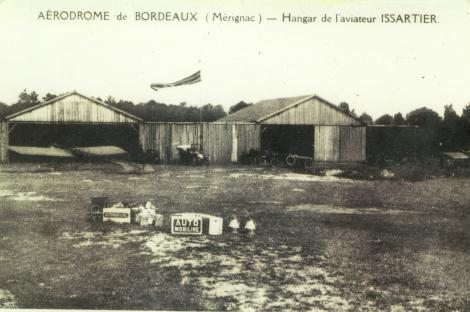
\includegraphics[width=.7\linewidth]{Images/premier.jpg}  
      \caption{Aérodrome de Bordeaux-Mérignac}
      \label{fig:aérodrome}
    \end{subfigure}
    \begin{subfigure}{0.5\textwidth}
      \centering
      % include second image
      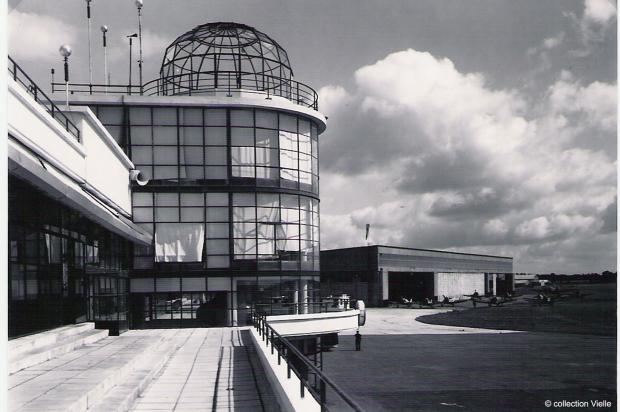
\includegraphics[width=.7\linewidth]{Images/premiere_aerogare.jpg}  
      \caption{Première Aérogare}
      \label{fig:premiereAerogare}
    \end{subfigure}
\end{figure}
De nombreux travaux se succèdent jusqu'en 2003 afin d'agrandir l'aéroport et d'y ajouter de nouveaux halls d'enregistrement et d'embarquements ainsi qu'une tour de contrôle.

En 2007, l'Etat concède l'exploitation et la gestion de l'aéroport à SA ADBM pour 30 ans. Depuis, de nombreux travaux ont été réalisés comme la création d'un nouveau parking plus économique, le hall "billi" destiné aux compagnies aériennes low-cost (Ryanair et EasyJet). Il sera par la suite agrandi en 2015.\newline

\begin{figure}[hbt!]
    \begin{subfigure}{0.5\textwidth}
      \centering
      % include first image
      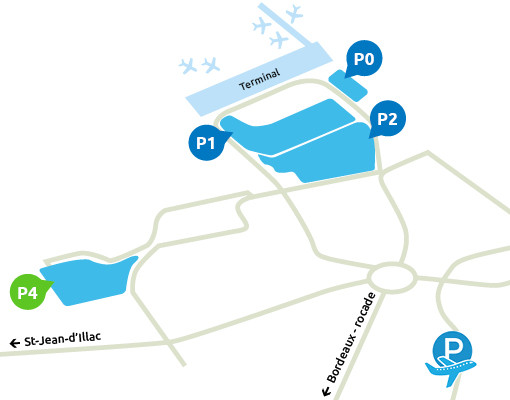
\includegraphics[width=.7\linewidth]{Images/parkings.jpg}  
      \caption{Plan des parkings}
      \label{fig:parking4}
    \end{subfigure}
    \begin{subfigure}{0.5\textwidth}
      \centering
      % include second image
      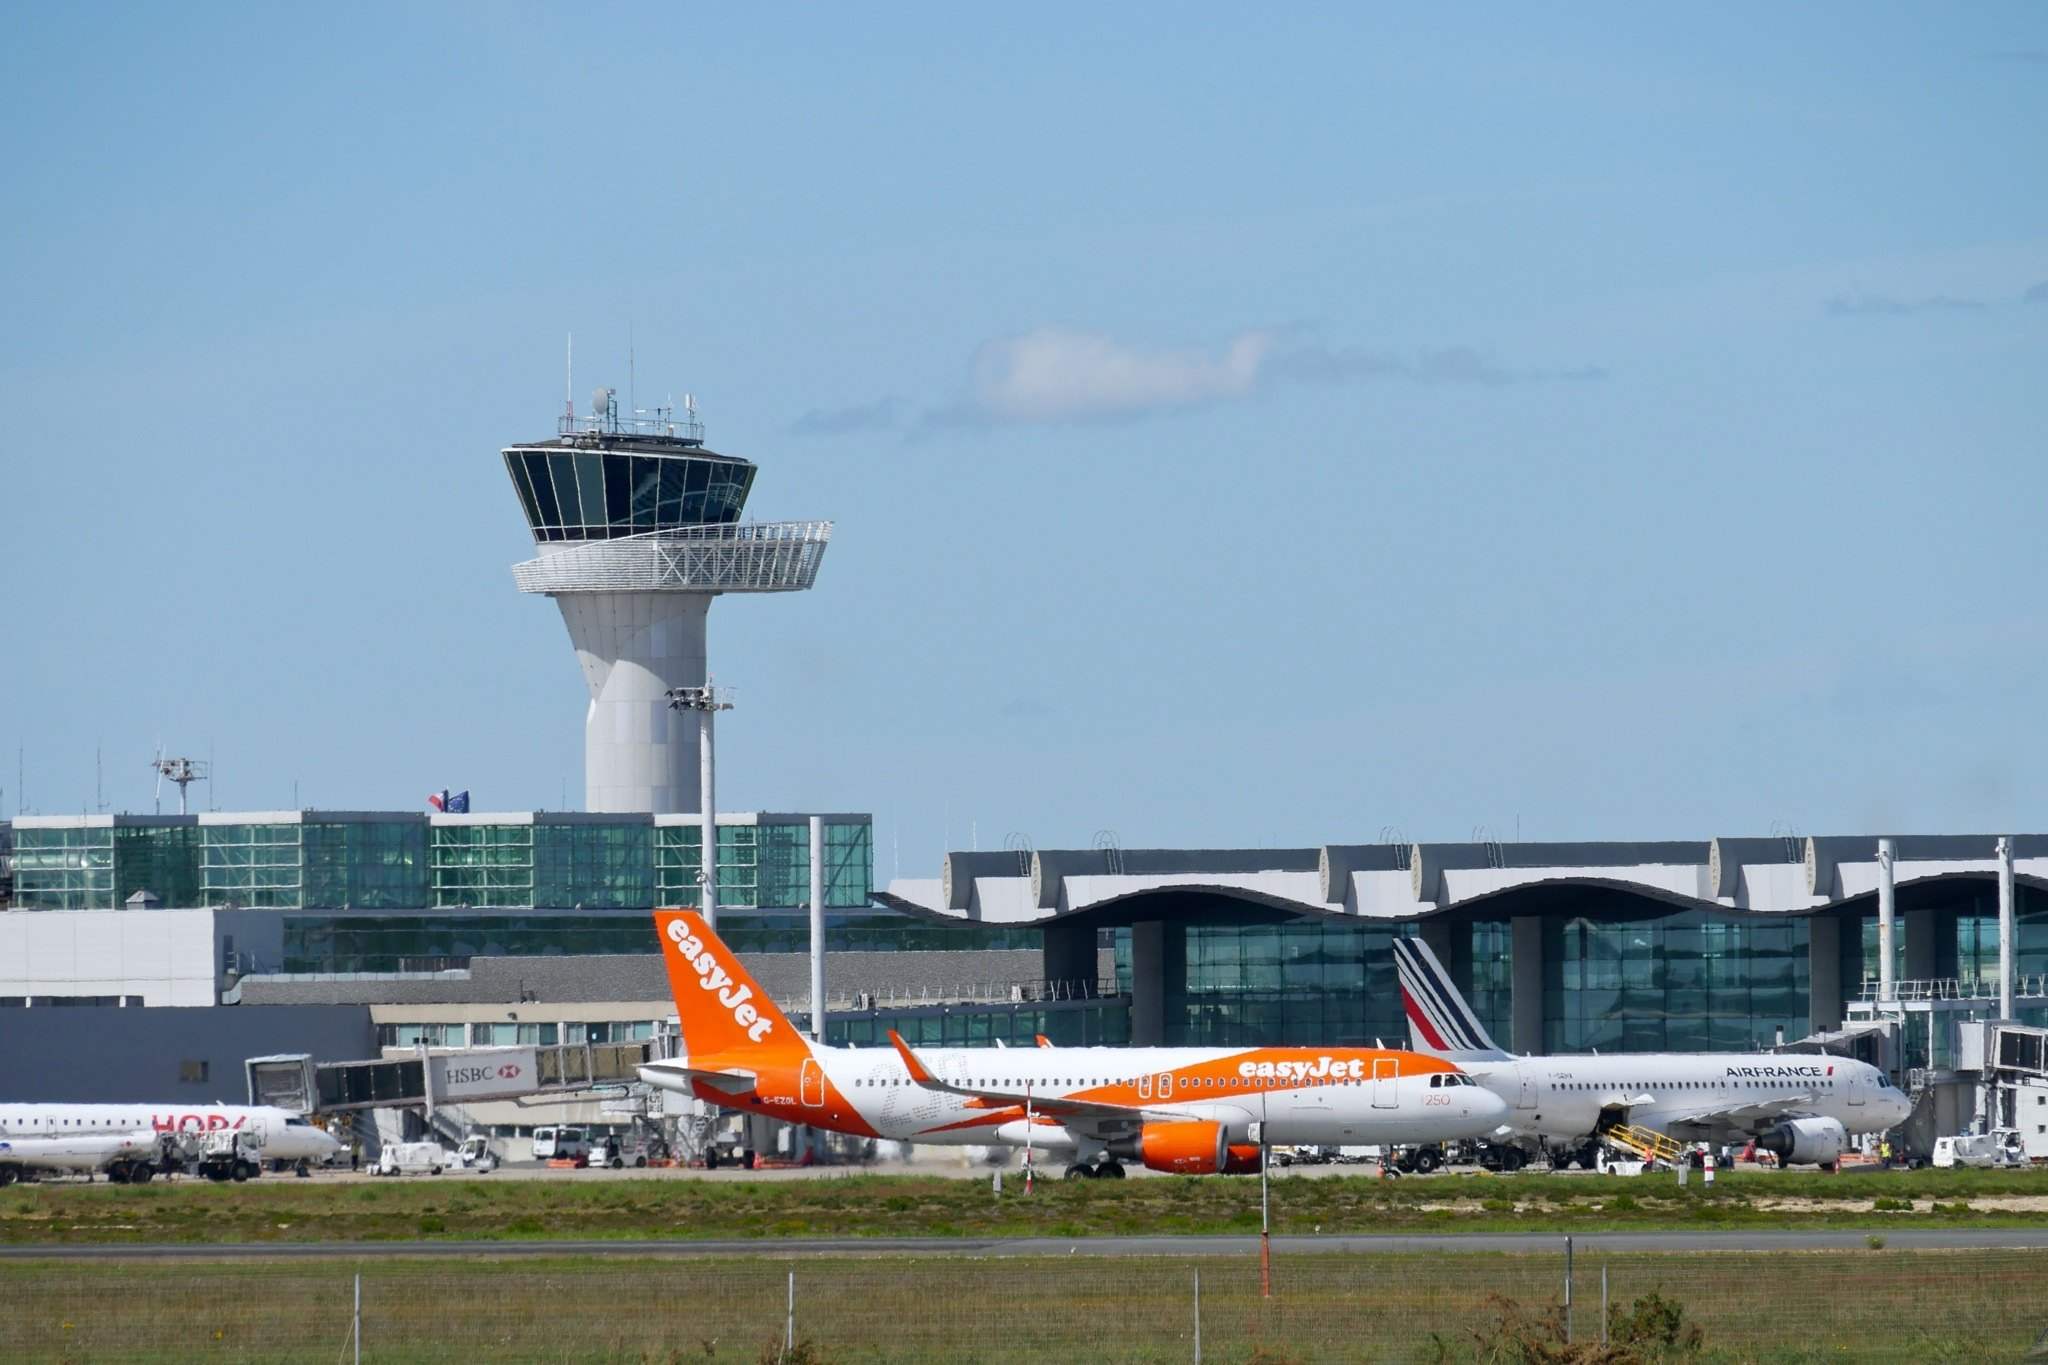
\includegraphics[width=.7\linewidth]{Images/tour.jpg}  
      \caption{Nouvelle Tour de Contrôle}
      \label{fig:tour}
    \end{subfigure}
        
    \begin{subfigure}{.5\textwidth}
      \centering
      % include third image
      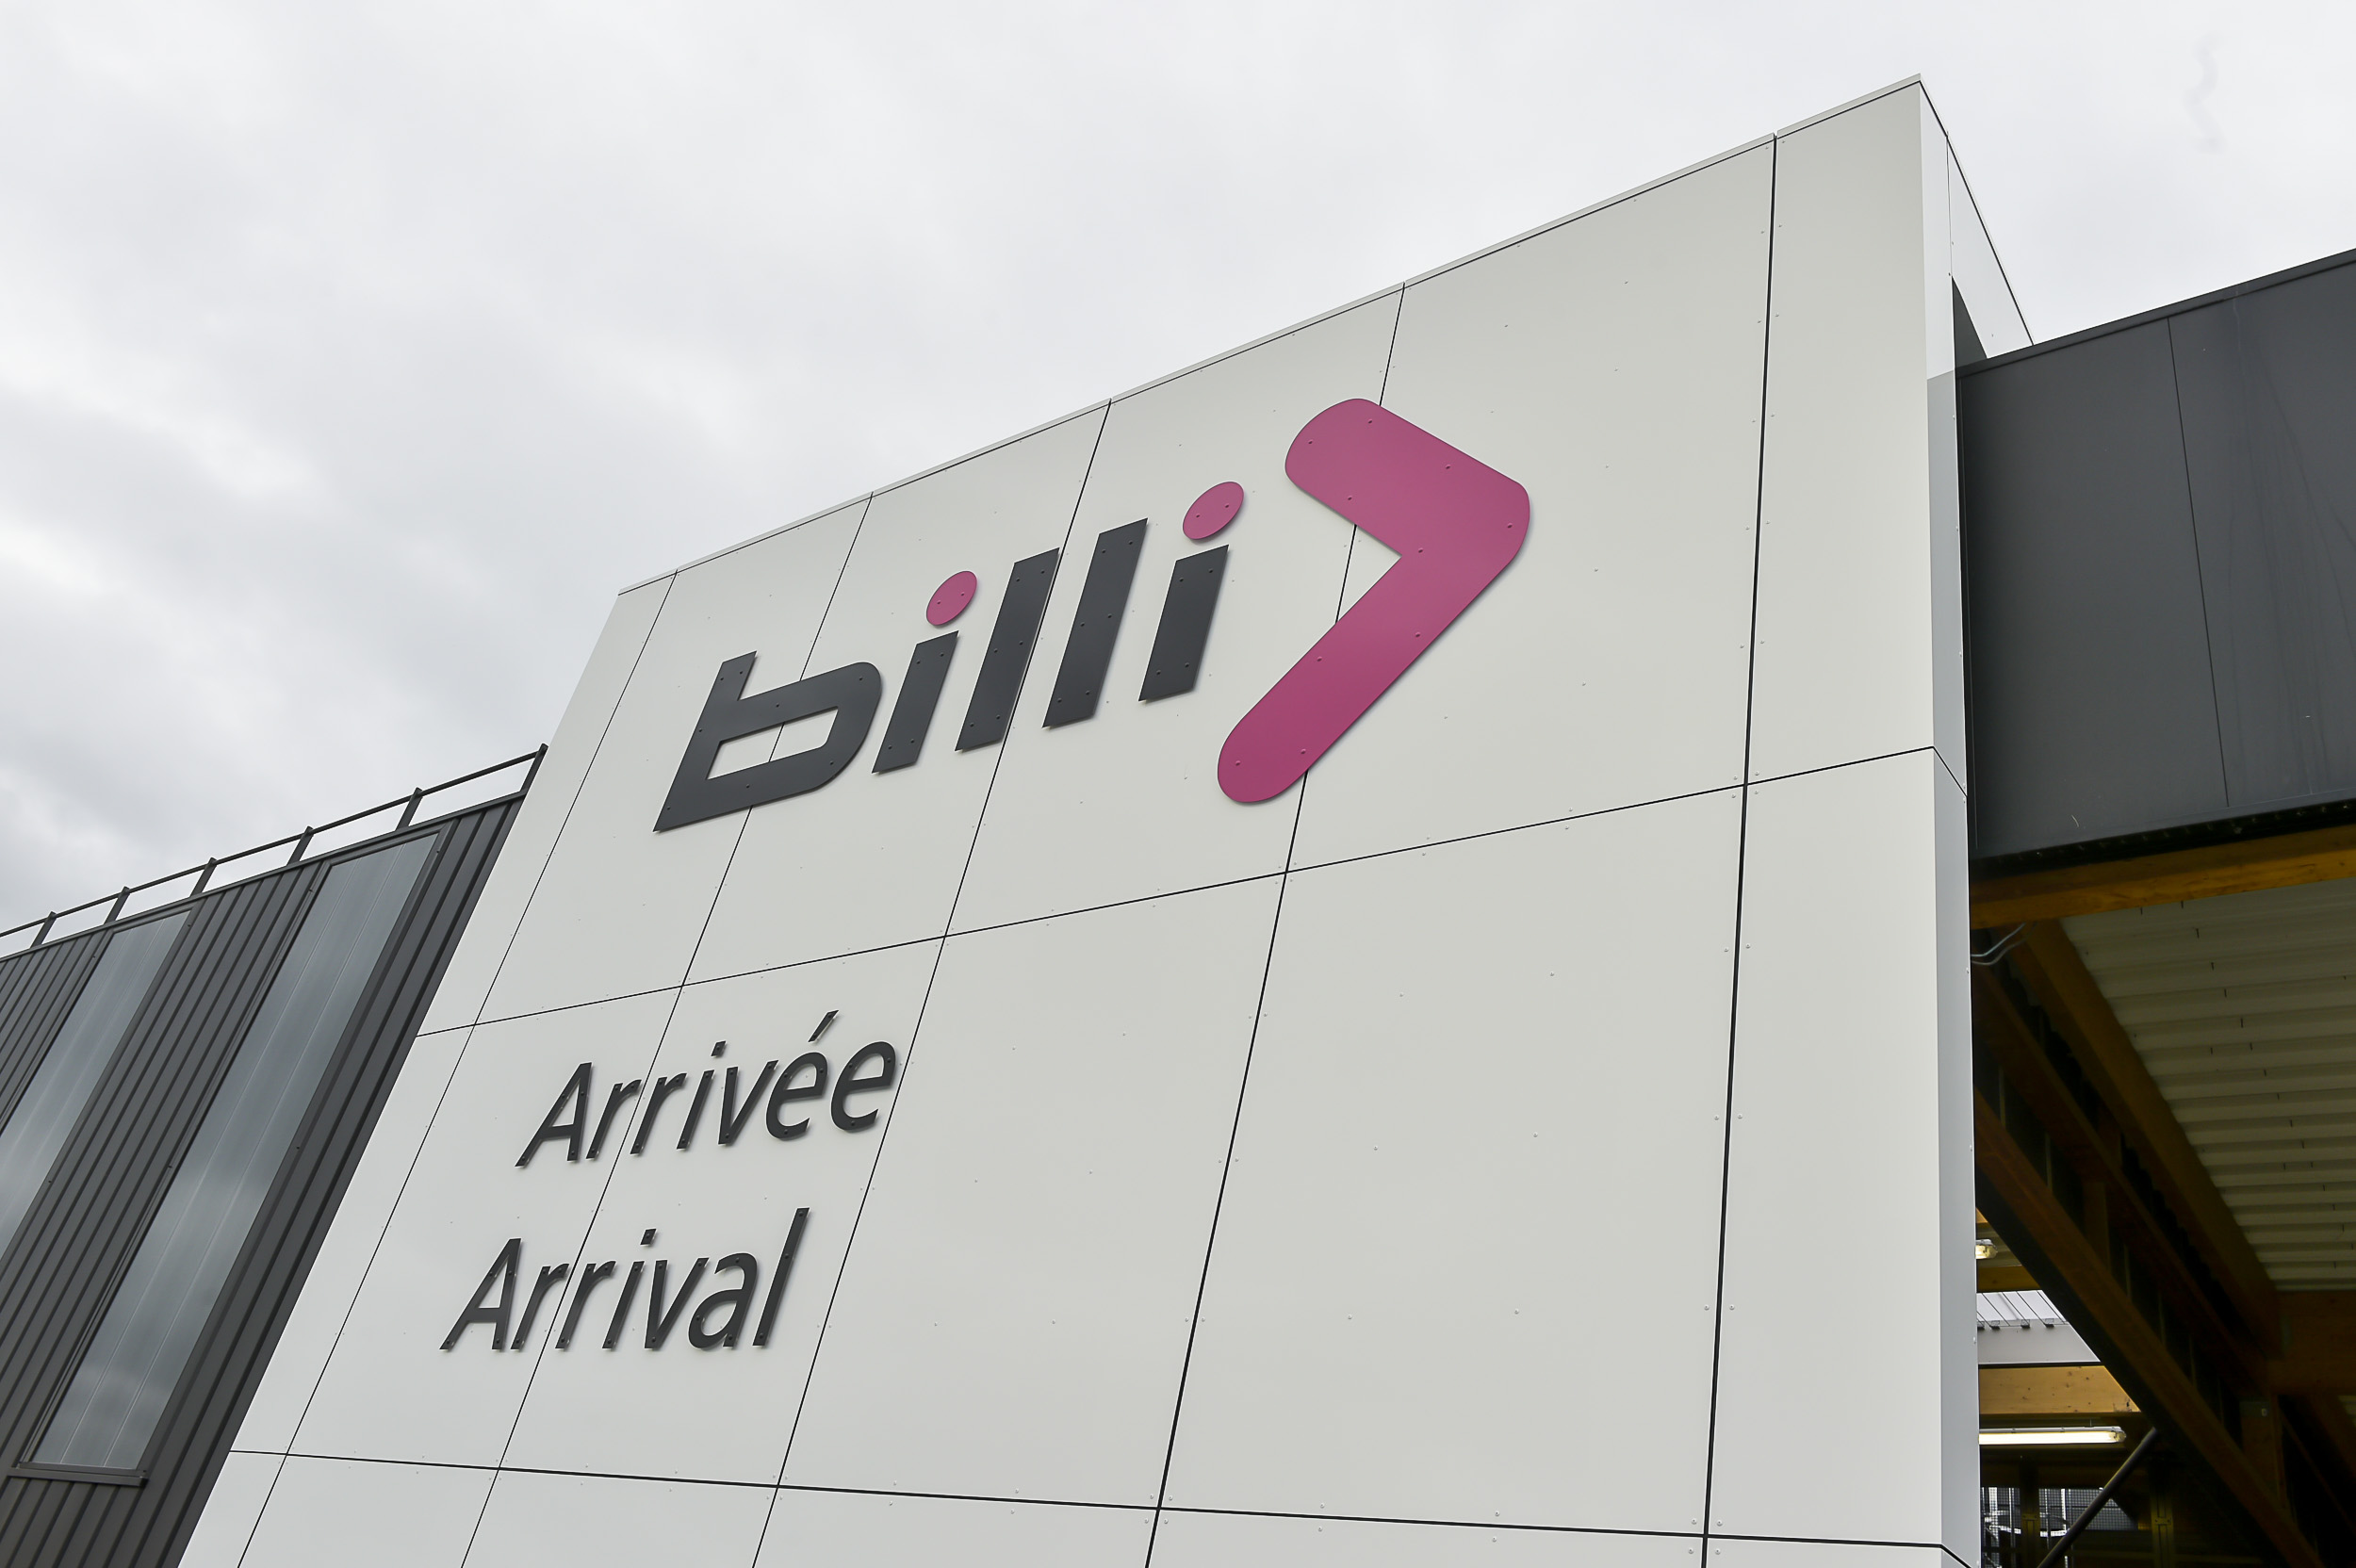
\includegraphics[width=.7\linewidth]{Images/billiext.jpg}  
      \caption{Terminal Billi}
      \label{fig:billiext}
    \end{subfigure}
    \begin{subfigure}{.5\textwidth}
      \centering
      % include fourth image
      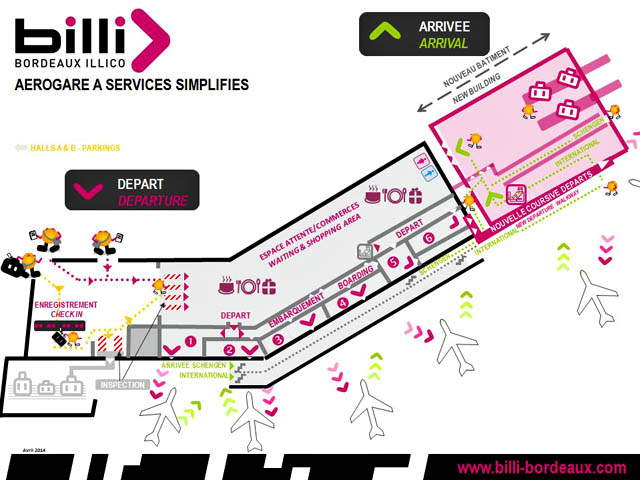
\includegraphics[width=.7\linewidth]{Images/billi.jpg}  
      \caption{Plan Billi}
      \label{fig:planBilli}
    \end{subfigure}
    \label{fig:travaux}
\end{figure}


\textbf{Infrastructures actuelles}\newline


A ce jour, la SA ADBM gère et exploite toujours l'Aéroport de Bordeaux-Mérignac.
L'aéroport possède aujourd'hui 2 pistes sécantes, 39 portes d'embarquements et 3 terminaux :

\begin{itemize}
    \item Le Hall A : National et International
    \item Le Hall B : National AirFrance uniquement
    \item Billi : National et International Low-Cost uniquement (EasyJet et Ryanair)
\end{itemize}

Les Hall A et B possèdent deux niveaux accessibles au public, le niveau 0 pour les arrivées et le niveau 1 pour les départs.

\begin{figure}[hbt!]
    \begin{subfigure}{0.5\textwidth}
      \centering
      % include first image
      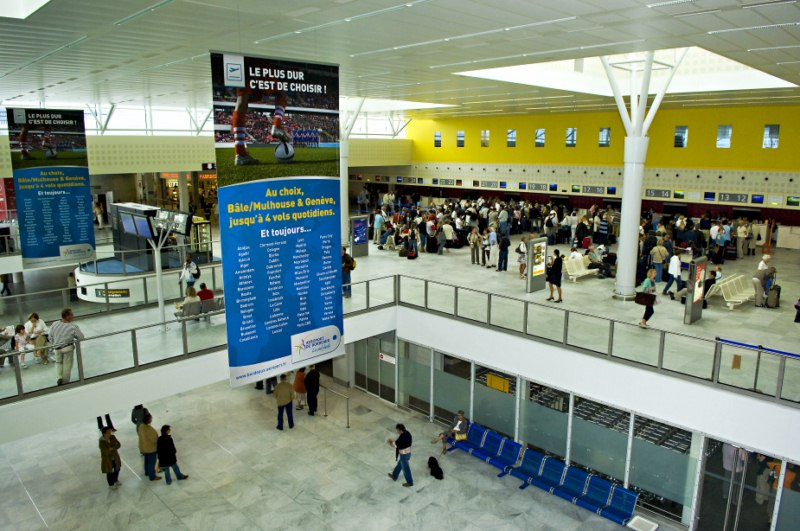
\includegraphics[width=.7\linewidth]{Images/inthalla.jpg}  
      \caption{Intérieur Hall A}
      \label{fig:inthalla}
    \end{subfigure}
    \begin{subfigure}{0.5\textwidth}
      \centering
      % include second image
      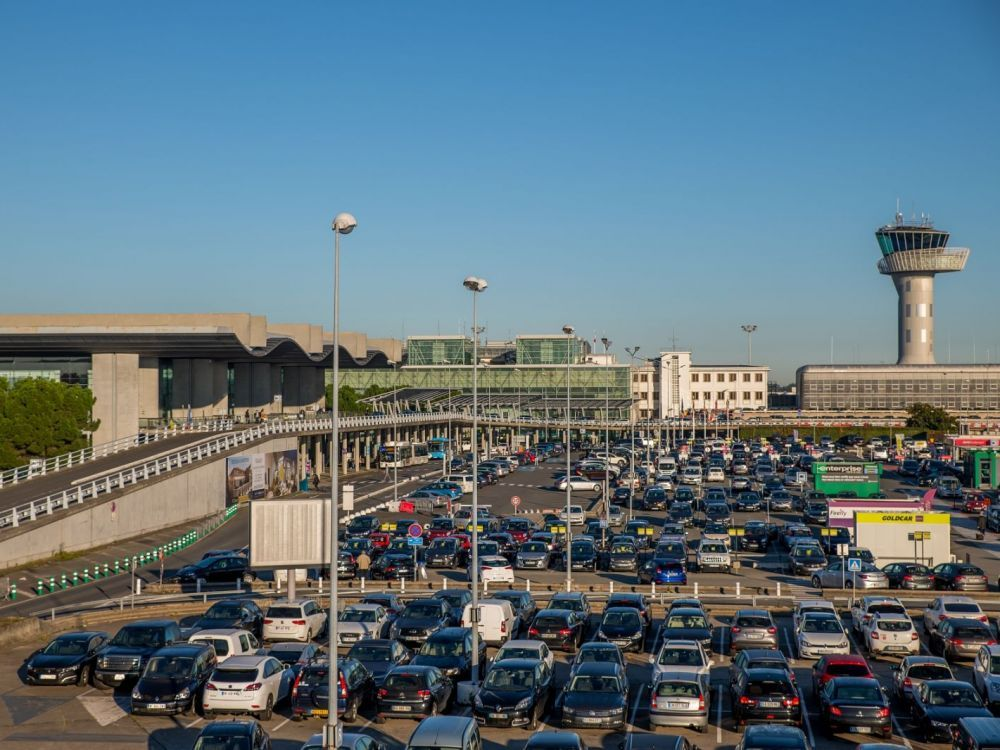
\includegraphics[width=.7\linewidth]{Images/exthalla.jpg}  
      \caption{Extérieur Hall A}
      \label{fig:exthalla}
    \end{subfigure}
        
    \begin{subfigure}{.5\textwidth}
      \centering
      % include third image
      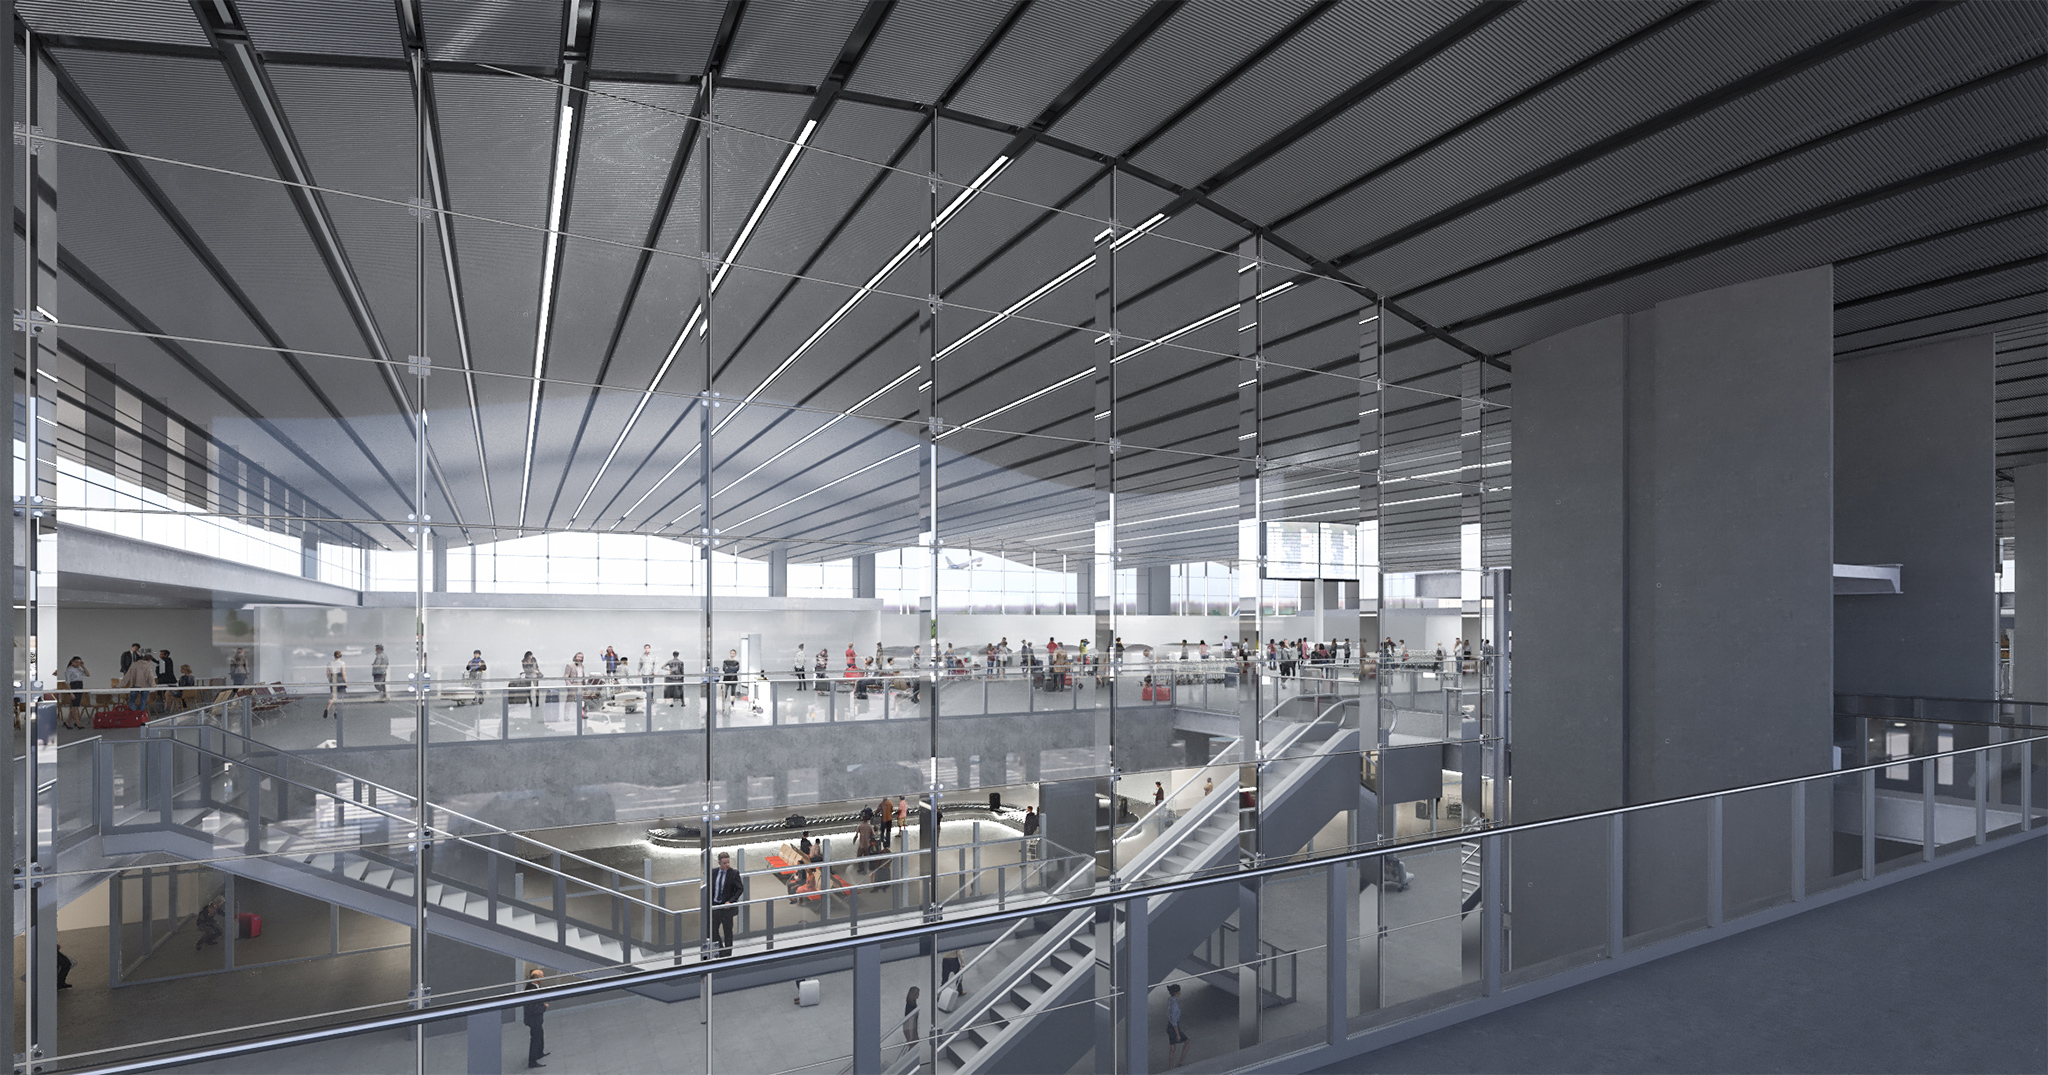
\includegraphics[width=.7\linewidth]{Images/inthallb.jpg}  
      \caption{Intérieur Hall B}
      \label{fig:inthallb}
    \end{subfigure}
    \begin{subfigure}{.5\textwidth}
      \centering
      % include fourth image
      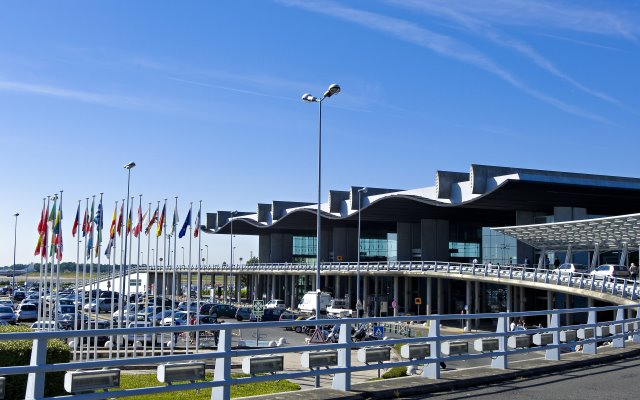
\includegraphics[width=.7\linewidth]{Images/exthallb.jpg}  
      \caption{Extérieur Hall B}
      \label{fig:exthallb}
    \end{subfigure}
    \caption{Les différents Halls}
    \label{fig:halls}
\end{figure}

\begin{figure}[hbt!]
    \centering
    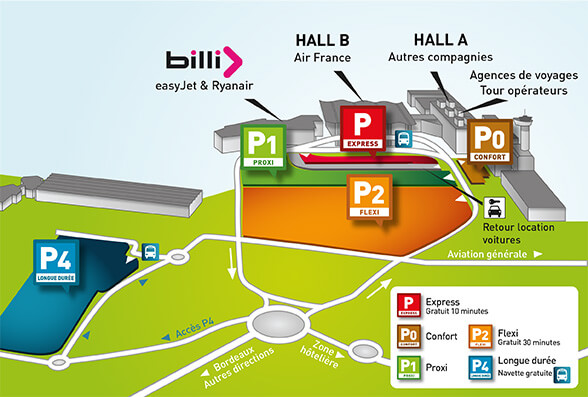
\includegraphics[width=.7\linewidth]{Images/plan.jpg}
    \caption{Plan Général}
    \label{fig:plangeneral}
\end{figure}

\newpage

\textbf{Infrastructures futures}\newline

Actuellement, deux plans d'aménagement on été engagés : Le Satellite 3 et le prolongement de la ligne A du Tramway.

Le Satellite 3 est un nouveau bâtiment construit côtés pistes du Hall A afin d'augmenter le nombre de portes d'embarquements pour l'international.

La livraison de ce bâtiment est prévue pour fin août 2021.\newline

\begin{figure}[hbt!]
    \centering
    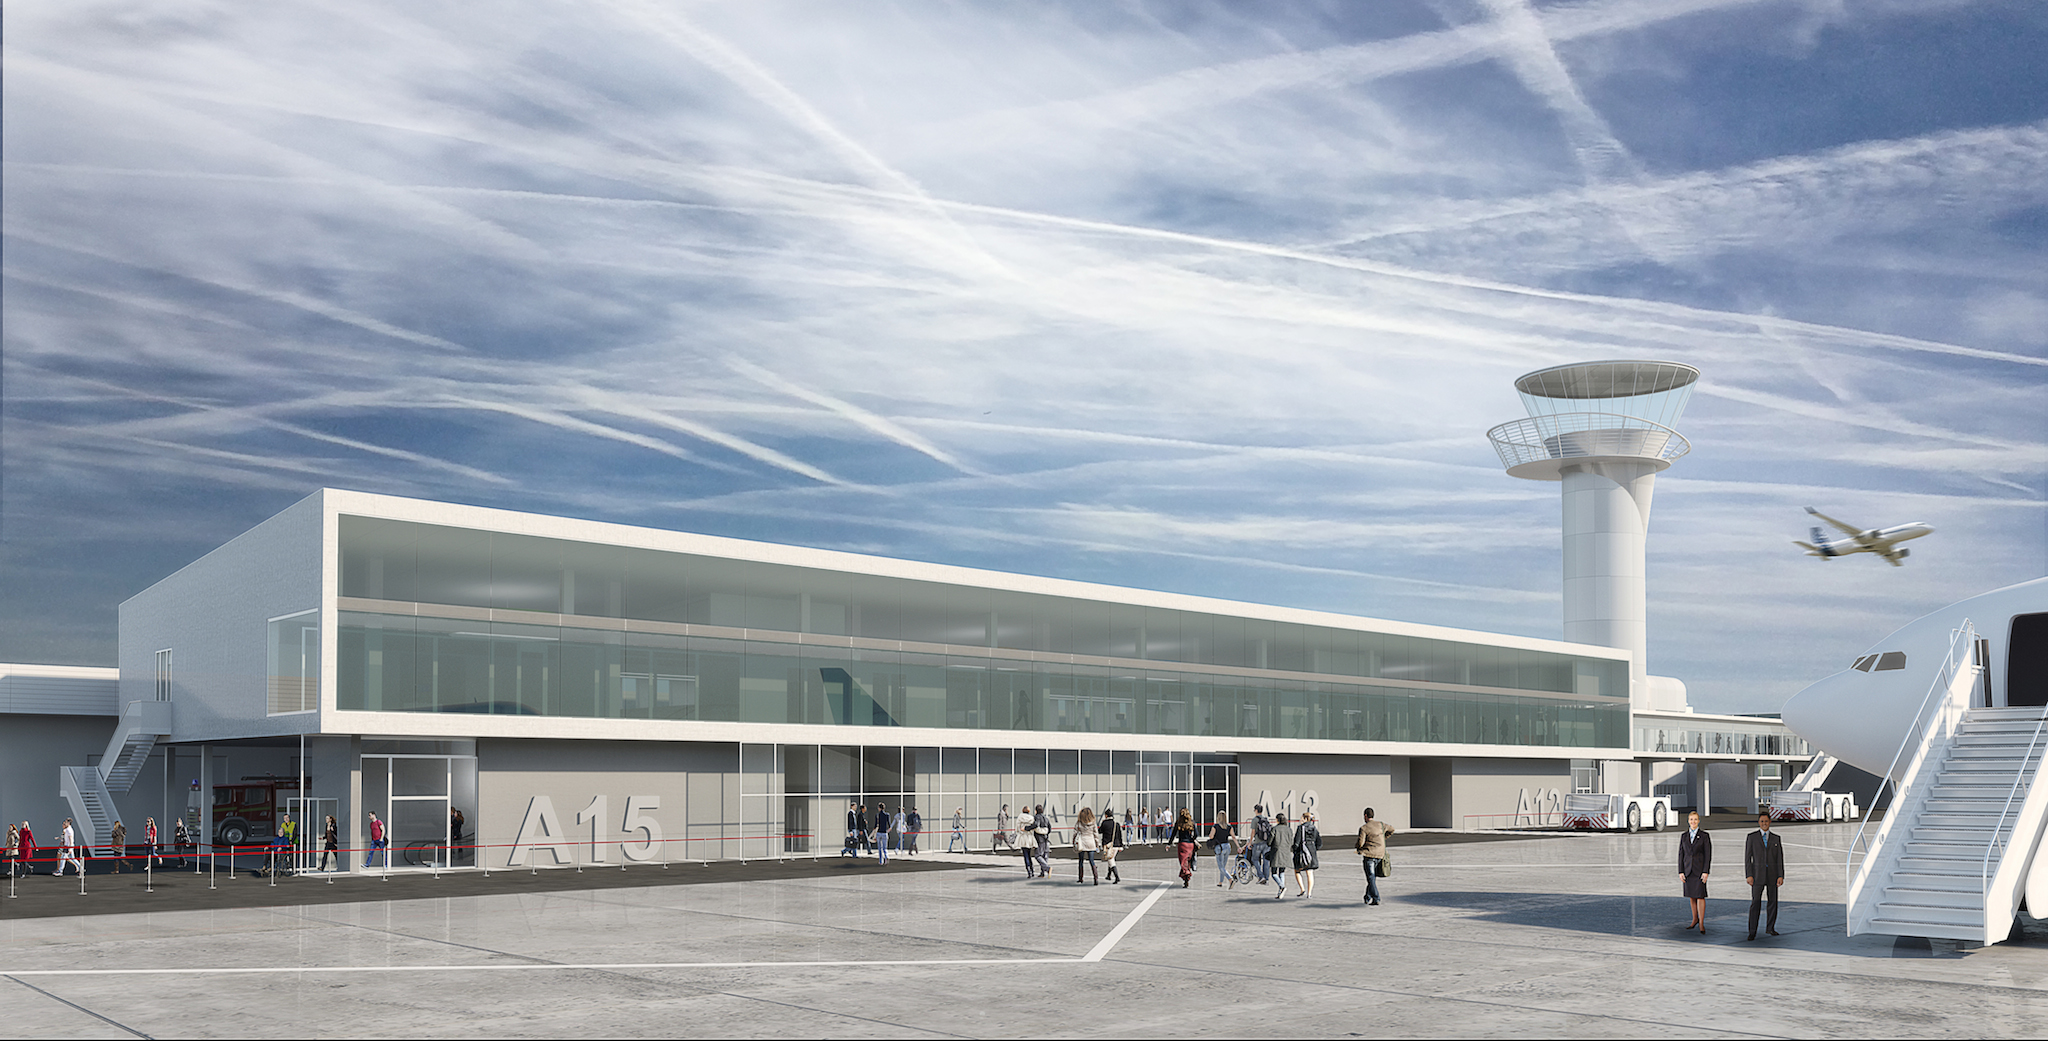
\includegraphics[width=12cm]{Images/satellite3.jpg}
    \caption{Futur Satellite 3}
    \label{fig:sat3}
\end{figure}

En partenariat avec Bordeaux Métropole, SA ADBM a engagé des travaux qui visent à rendre l'accès à l'aéroport plus simple. La ligne de tram A est donc prolongée de 6 stations avec le Terminus au pied des aéroports. Ces travaux ont été lancés en 2019 et la livraison est prévue pour automne 2022.\newline

\begin{figure}[hbt!]
    \centering
    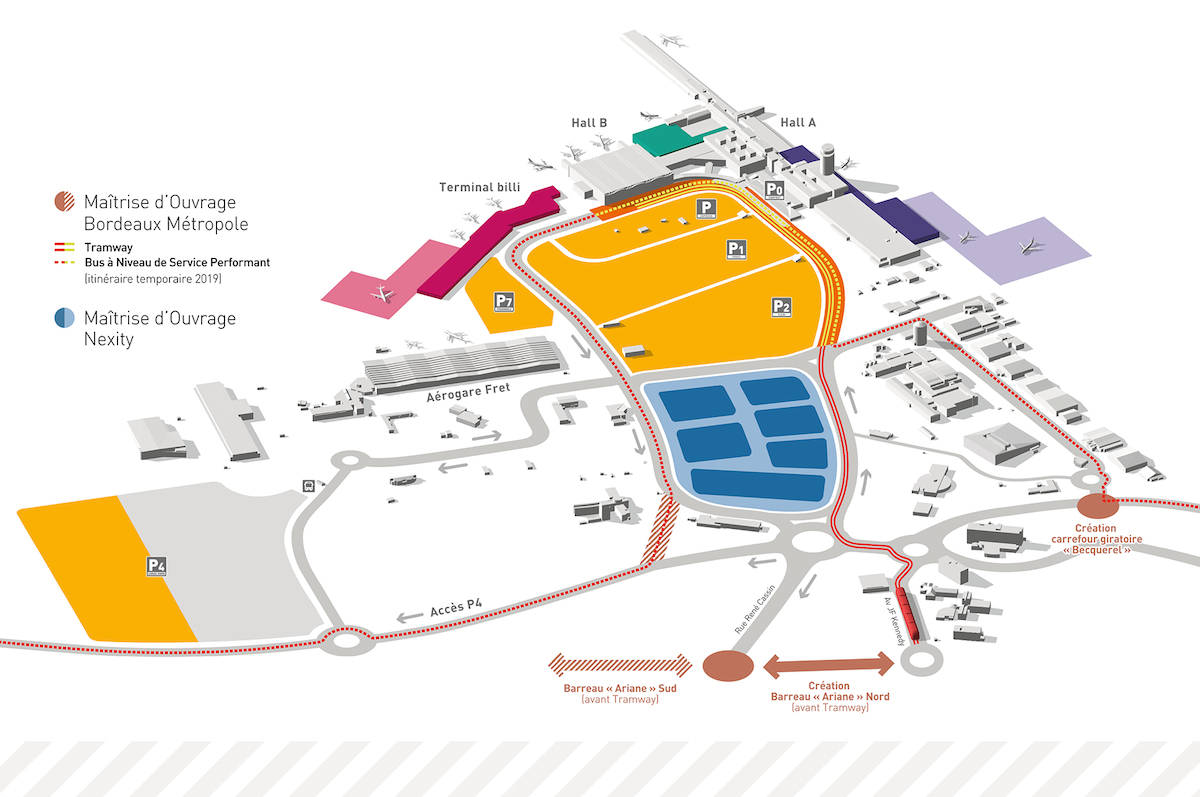
\includegraphics[width=14cm]{Images/tramway.jpg}
    \caption{Plan Futur Tram}
    \label{fig:futurtram}
\end{figure}

\newpage

\textbf{Chiffres clés}\newline

L'aéroport de Bordeaux-Mérignac a fait voyager près de 7,7 millions de passagers en 2019. Cela correspond à une croissance +134\% par rapport à 2018 :

\begin{figure}[hbt!]
    \centering
    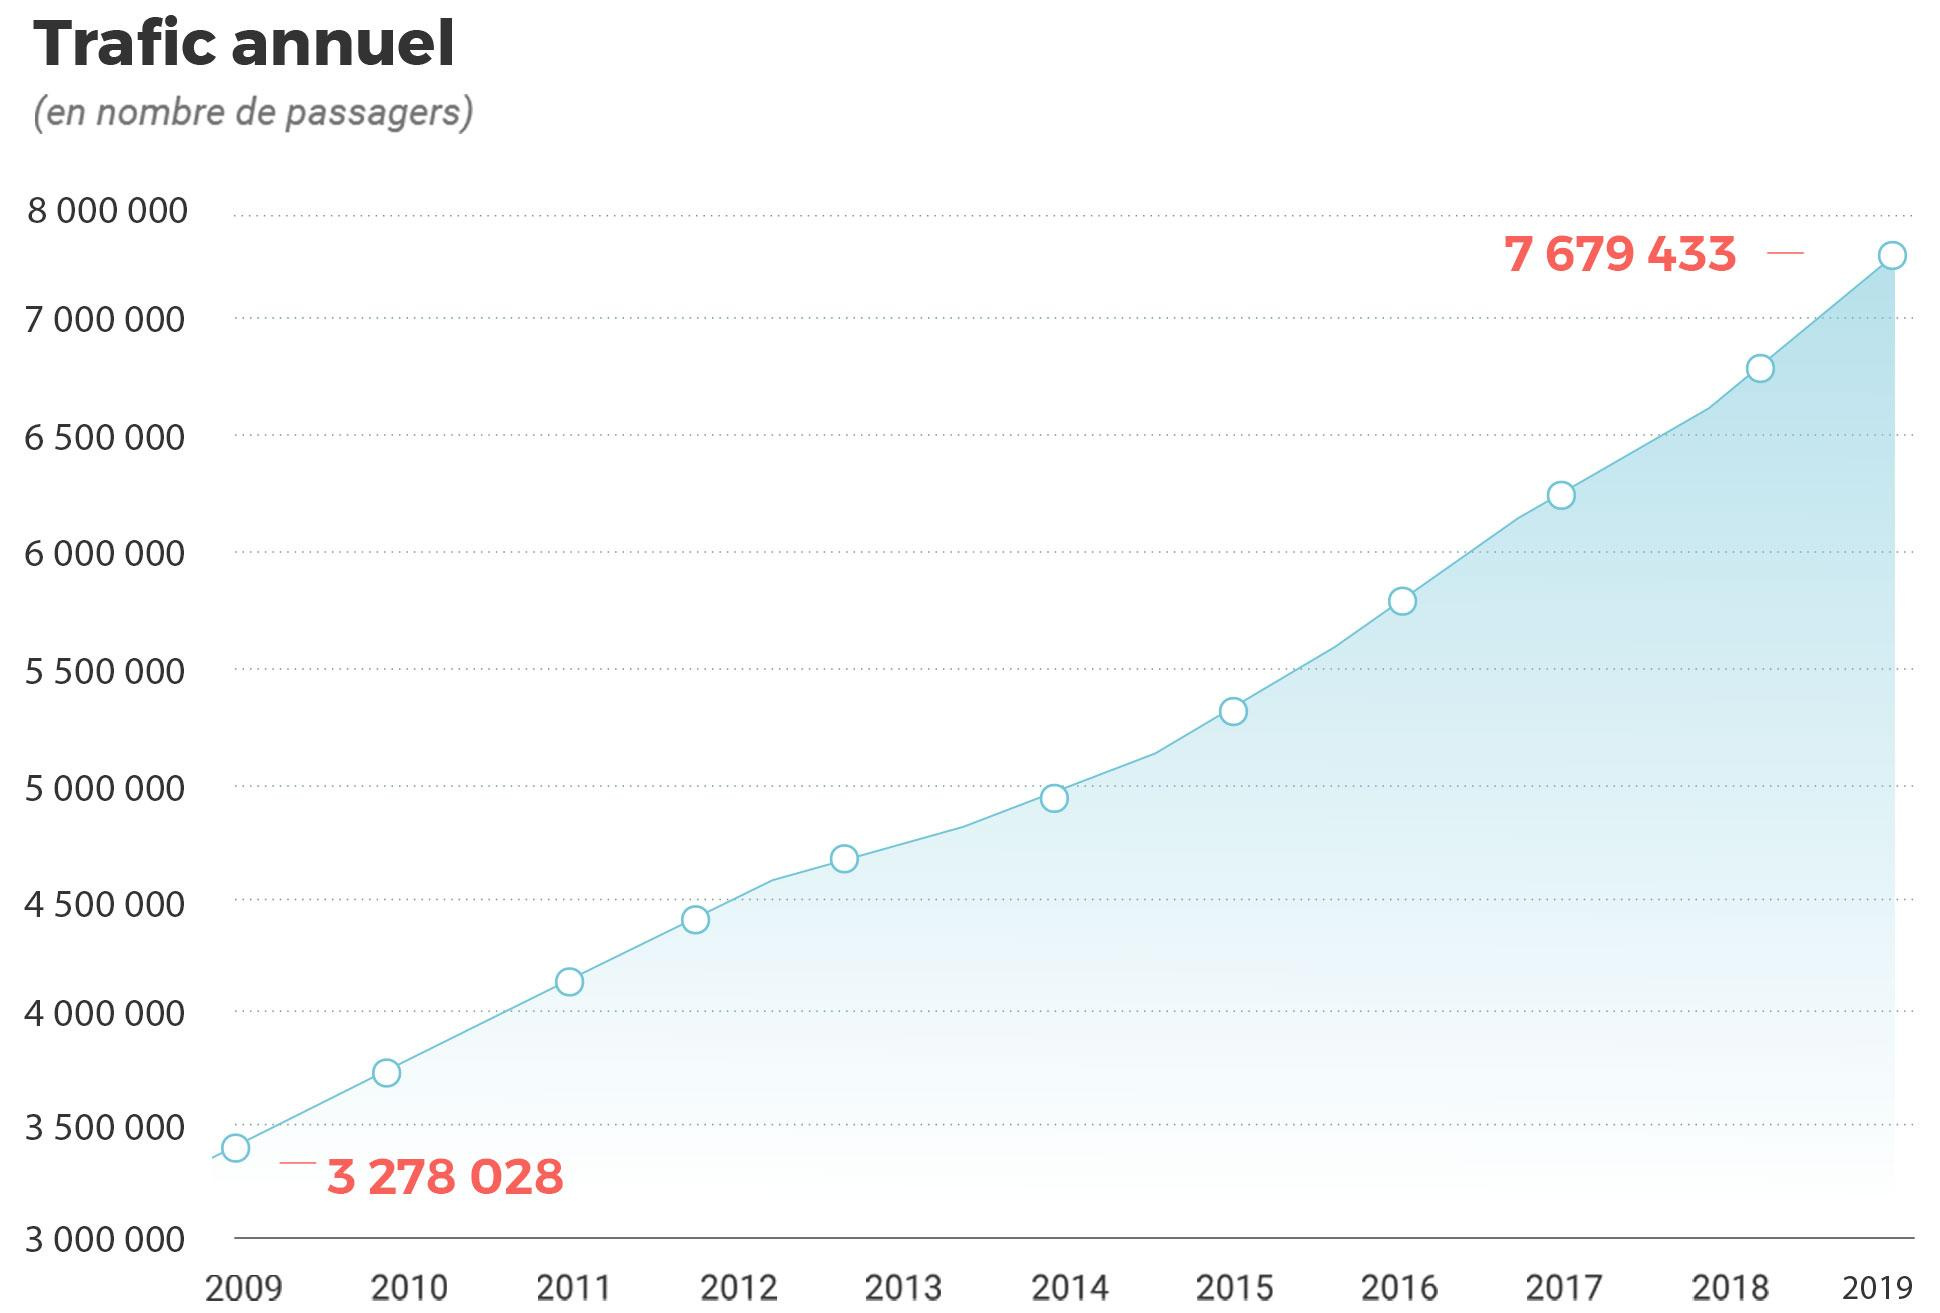
\includegraphics[width=12cm]{Images/trafic.jpg}
    \label{fig:trafic}
\end{figure}

Avant la pandémie de COVID-19, l'aéroport avait pour but de faire voyager 10 millions de passagers en 2023.

En 2019, 34 compagnies aériennes ont opéré des vols, avec un total de 163 lignes directes reliées à 31 pays différents.
De plus, plus de 125 000 tonnes de fret ont été acheminées grâce aux cargos.

C'est également un bassin d'emploi important puisque plus de 8000 personnes travaillent sur la plateforme aéroportuaire (dont 200 SA ADBM).
94 établissements sont présents sur site : entreprises, commerces, industries et organismes publics.

\subsubsection*{Personnes impliquées}


Mon tuteur était Serge CLARY, Chef de Projet Informatique, et ma supérieure Nathalie CORDEAU, Chef du Service Organisation, Informatique, Systèmes Industriels au sein du département.\footnote{Tous les organigrammes disponibles en Annexe}

J'ai travaillé en proche collaboration avec :\newline

\begin{itemize}
    \item Monsieur Marc RIVAULT : Administrateur Systèmes, Réseaux et Bases de données,
    \item Monsieur Gurvan QUENET : Responsable Sécurité des Systèmes d'Information,
    \item Monsieur Kamal MAHAMOUD : Technicien Support Informatique,
    \item Monsieur Yannick VALERY : Administrateur Systèmes, Réseaux et Bases de données.
\end{itemize}

J'ai également été reçue par :

\begin{itemize}
    \item Monsieur CABANNE Olivier : Attaché Relations Riverains et Environnement,
    \item Madame COLAS Fabienne : Coordinateur Piste.
\end{itemize}


L'avantage d'une entreprise avec une grande variété de postes, est que j'ai pu constater à quel point l'informatique est essentiel dans tous les services, autant sur l'aspect logiciel que matériel.

\subsubsection*{Activités}

Les salariés de l'aéroport étant toujours sur Office 2010, ma première mission a été d'analyser les différences entre Office 2010 et 2019 afin de savoir quel type de formation ou documentation pourrait accompagner la transition, et ensuite de la réaliser.
J'ai donc créé un document détaillé de tous les changements entre ces versions, puis ensuite un "flyer" les résumant de manière simplifiée.\newline

Ma seconde mission était de mettre à jour des ordinateurs "CREWS", les passer de Windows 7 à Windows 10 en réinstallant d'autres logiciels. En banque d'enregistrement, ce sont des ordinateurs qui permettent d'enregistrer les bagages en soute et d'imprimer leurs identifications à partir d'un scan de la carte d'embarquement du passager.
J'ai commencé à faire quelques manipulations sur les ordinateurs CREWS : Mise à jour du BIOS, Installation de Windows à partir d'un logiciel de gestion : Ivanti.
Cependant je n'ai jamais pu les installer, des problèmes techniques ont été repérés plus tard dans l'installation, et nous avons donc dû suspendre le projet.\newline

Durant le premier confinement, certains salariés se sont vus attribués un ordinateur portable afin de faire du télétravail. Or plusieurs vols ont été enregistrés chez ces personnes, et au délà de la perte financière, la perte du disque dur représentait une perte d'informations internes et donc un problème de sécurité.
Il fallait donc régler le problème afin de ne pas risquer une fuite de données, CRYHOD était la solution. CRYHOD est un logiciel de cryptage de données de disques durs.
Gurvan QUENET, le Responsable Cybersécurité de l'aéroport m'a donc donné la mission d'installer ce logiciel sur les ordinateurs portables des salariés afin de sécuriser les disques durs et protéger les données de l'aéroport.
J'ai pu l'effectuer sur quelques postes, mais Monsieur QUENET m'a demandé d'arrêter à cause d'un problème de compatibilité sur certains logiciels, la mise en place a donc été retardée.\newline

Enfin, après l'annonce du confinement national en mars 2020, des outils informatiques ont été prêtés : Postes, Ecrans, Périphériques.
Ma dernière mission était de passer dans tous les bureaux de l'aéroport et de recenser le matériel présent avant de comparer avec celui prêté dans la base de données afin de vérifier que tout le monde a bien ramené les outils prêtés.

\subsubsection*{Démarche Responsabilité Sociale de l’Entreprise}


Lorsque l'on pense à un aéroport ou même au milieu aéronautique en général, on ne pense pas à une bonne gestion de l'environnement.
Et pourtant, comme toute entreprise, l'Aéroport de Bordeaux-Mérignac pratique une politique RSE.


En effet, l'entreprise se rend compte que ses activités ont 